\section{Architektura hlubokého modelu variačního autoenkodéru}
Model variačního autoenkodéru se od prostého autoenkodéru (viz \autoref{chap:autoencoder}) liší zejména v \textbf{enkodér modulu} a \textbf{ztrátové funkci} (viz \autoref{sec:vae_objective}).
\subsection{Enkodér}
U prostého autoenkodéru je každý vstup mapován přímo na \textbf{pouze jeden bod} v latentním prostoru (tedy výsledný latentní prostor není spojitý).
Naopak ve variačním autoenkodéru je každý vstup mapován na (vícerozměrné) normální rozdělení okolo konkrétního bodu v latentním prostoru, jak ukazuje

\begin{figure}[H]
    \centering
    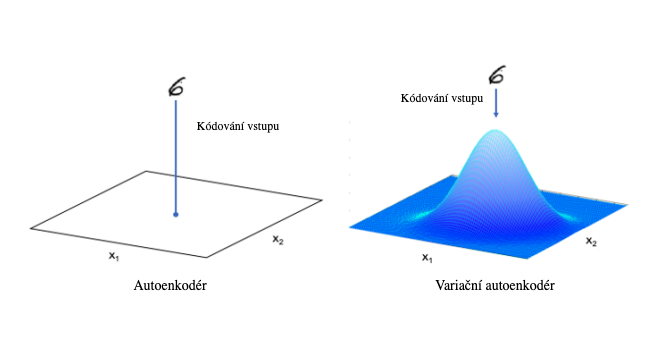
\includegraphics[width=\textwidth]{figures/vae_encoder_module.png}
    \caption{Rozdíl mezi enkodér modulem autoenkodéru a enkodér modulem variačního autoenkodéru. Umožňuje vzorkování ze spojitého latentního prostoru VAE. Obrázek převzat z \textcite{Foster2023}}.
    \label{fig:vae_encoder_difference}
\end{figure}

Pro připomenutí, jak plyne z \autoref{sec:vae_encoder}, enkodér modul variačního autoenkodéru \textbf{zakóduje každý vstup do dvou vektorů} – $mu$ a $log_var$
\footnote{Jak víme z \autoref{sec:vae_optimization} enkodér modul předpokládá že \textbf{neexistuje korelace mezi žádnou z dimenzí latentního prostoru} a tím pádem je výsledná kovarianční matice diagonální. V důsledku tak enkodér modulu stačí mapovat každý vstup na vektor středních hodnot a vektor rozptylu.},
ze kterých je následně v latentním prostoru \textbf{sestaveno} (vícerozměrné) \textbf{normální rozdělení}, kde:\\
$mu$: Střední hodnota rozdělení a $log_var$: logaritmus rozptylu každé dimenze.\\

Pro vytvoření kódu vstupního obrázku do konkrétní latentní proměnné $z$ v latentním prostoru modelu lze z takto vzniklé distribuce vzorkovat pomocí následujícího vztahu:\\
$z = mu + sigma * epsilon$, kde $sigma = exp(log_var / 2)$ \\
a $epsilon$ je bod vzorkovaný z normovaného normálního rozdělení.

Tento princip enkodér modulu je velmi důležitý, jelikož zprostředkovává \textbf{spojitost latentního prostoru pro účely vzorkování}.
Vraťme se k prostému autoenkodéru (viz \autoref{chap:autoencoder}) – jeho latentní prostor není spojitý.
Pakliže bychom vytvořili model pouhého autoenkodéru, např. bod $(1.5, -2.5)$ v jeho latentním prostoru by bylo možné rozkódovat na dobře formovaný obrázek číslice $1$, není ale zaručeno že bod $(1.6, -2.6)$ by byl rovněž rekonstruován na obrázek \emph{podobný} této číslici (ve skutečnosti by taková rekonstrukce pravděpodobně vůbec nebyla definována).

Jak napovídá \autoref{fig:vae_encoder_difference}, enkodér modul variačního autoenkodéru ale tento problém řeší.
Jelikož je vzorkován náhodný bod z okolí $mu$, dekodér \textbf{musí zajistit} že chyba rekonstrukce všech bodů v jeho okolí bude nízká.
Toto je vlastnost, která zaručuje že i když zvolíme bod v latentním prostoru, který doposud nebyl dekodérem spatřen, je vysoká pravděpodobnost že tento bod bude rekonstruován na obrázek který bude \emph{podobný} očekávanému vstupu.
Toto je způsob, kterým \textbf{variační autoenkodér generuje syntetická data}, která zachycují charakteristiky vstupních dat, ale nebyly součástí trénovací množiny.

\lstinputlisting[language=Python, caption=Kód enkodér modulu VAE]{code_snippets/encoder.py}

Má za výsledek následující enkodér modul:
\begin{figure}[H]
    \centering
    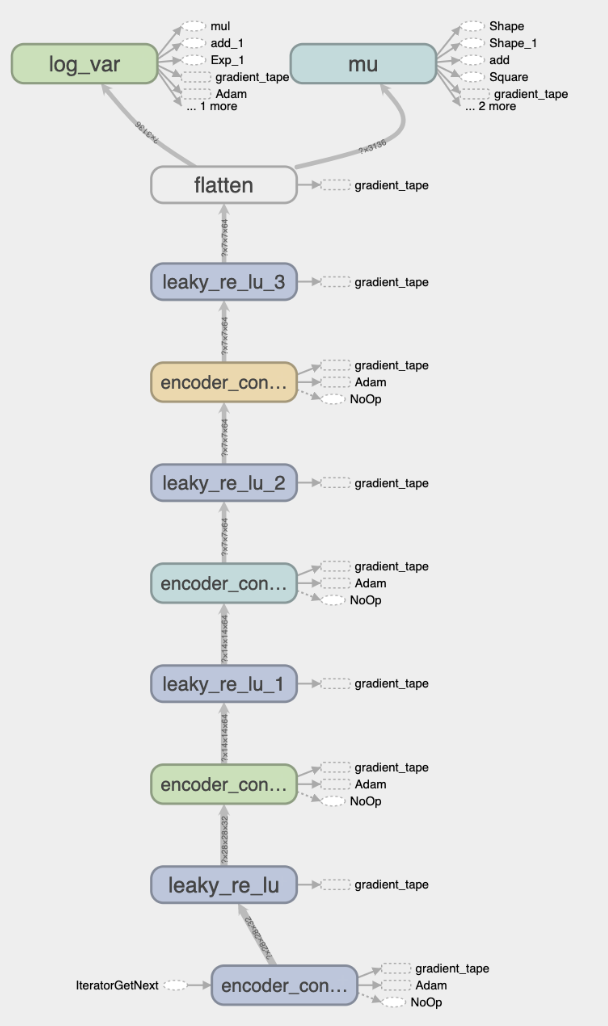
\includegraphics{figures/vae_model_encoder.png}
    \caption{Diagram enkodér modulu VAE pro generování MNIST číslic.}
    \label{fig:vae_model_encoder}
\end{figure}

\subsection{Dekodér}
Dekodér modul variačního autoenkodéru je principem identický k dekodéru prostého autoenkodéru.

\subsection{Reparametrizační trik}
\lstinputlisting[language=Python]{code_snippets/vae_reparametrization.py}

\subsection{Ztrátová funkce}
Ztrátová funkce modelu variačního autoenkodéru implementuje postup dle \autoref{eq:vae_elbo}.
Model VAE tedy \textbf{minimalizuje součet hodnoty chyby rekonstrukce a hodnoty KL divergence}.

Připomeňme z \autoref{sec:kl_divergence}, že KL divergence vyjadřuje míru nepodobnosti (resp. \emph{"vzdálenosti"}) mezi pravděpodobnostními distribucemi.
U variačního autoenkodéru chceme měřit jak moc se liší normální rozdělení s parametry \lstinline{mu} a \lstinline{log_var} oproti normovanému normálnímu rozdělení.
Prvek KL divergence tedy penalizuje umělou neuronovou síť modelu za takové kódování vstupních dat (jehož výsledkem je \lstinline{mu} a \lstinline{log_var}), které se \textbf{výrazně liší} od parametrů normované normálního rozdělení.
Tento prvek KL divergence tak hraje při trénování modelu důležitou roli, jelikož \emph{nutí} všechny distribuce s parametry, které jsou výsledkem kódování, \emph{podobat se} normovanému normálnímu rozdělení. 
V důsledku existuje \textbf{menší šance} že zformovaný \textbf{latentní prostor model bude obsahovat} \emph{značné} \textbf{mezery} mezi klastry latentních proměnných (jak ukazuje \autoref{sec:vae_model_latent_space_observation}).
Ve snaze o minimalizaci ztrátové funkce modelu se totiž enkoder modul pokouší o efektivní a symetrické využití prostoru v okolí počátku latentního prostoru.

Ztrátová funkce rovněž musí hledat \textbf{rovnováhu mezi hodnotou chyby rekonstrucke a hodnotou KL divergence}.
Udělení příliš velké váhy jednomu z těchto prvků by mělo za důsledek ztrátu kýženého regulačního efektu latentního prostoru a vzniklý model variačního autoenkodéru by nabýval stejných problémů, jako prostý autoenkodér.
Zajištění konvergence obou prvků je tak důležitou součástí trénovacího procesu modelu variačního autoenkodéru a vede k chtěné vlastnosti spojitého latentního prostoru, která umožňuje variačnímu autoenkodéru generovat i takové vzorky dat, které nebyly součástí trénovací množiny.

\newpage
\lstinputlisting[language=Python]{code_snippets/vae_loss_function.py}

Kde:
\begin{itemize}
    \item \lstinline{z_mean, z_log_var = self.encode(data)}: Volá enkodér modul VAE za účelem získání kódu vstupních dat (tedy parametrů pravděpodobnostní distribuce).
    \item \lstinline{z = self.reparameterization(z_mean, z_log_var)}: Realizuje \textbf{reparametrizační trik} dle \autoref{sec:reparametrization_trick} za účelem získání vzorku z latentního prostoru na základě parametrů jeho rozdělení pravděpodobnosti.
    \item \lstinline{reconstruction = self.decode(z)}: Generuje rekonstrukci vstupních dat (v tomto případě obrázku MNIST číslice) na základě získaných latentních proměnných voláním dekodér modulu VAE.
    \item \lstinline{reconstruction_loss = tf.reduce_mean(tf.reduce_sum(keras.losses.binary_crossentropy(data, reconstruction), axis=(1, 2)))}: Realizuje gradientní optimalizaci dle \autoref{eq:vae_final_objective} výpočtem chyby rekonstrukce vygenerovaného vzorku vůči vstupním datům.
    \item \lstinline{kl_loss = -0.5 * (1 + z_log_var - tf.square(z_mean) - tf.exp(z_log_var))}: Spočte KL divergenci mezi pravděpodobnostní distribucí latentních proměnných (s parametry \lstinline{z_mean}, \lstinline{z_log_var} ) a normovaným normálním rozdělením.
    \item \lstinline{total_loss = reconstruction_loss + kl_loss}: Udává celkovou hodnotu ztrátové funkce dle \autoref{eq:vae_elbo}, respektive součet hodnoty chyby rekonstrukce a hodnoty KL divergence.
    \item \lstinline{grads = tape.gradient(total_loss, self.trainable_weights)}: Spočte gradienty vah dle \autoref{eq:vae_final_objective} s ohledem na celkovou hodnotu ztrátové funkce.
    \item \lstinline{self.optimizer.apply_gradients(zip(grads, self.trainable_weights))}: Stochastická gradientní optimalizace (s ohledem na spočtené gradienty) dle \autoref{alg:reparam_trick}.
\end{itemize}


